\documentclass[conference]{IEEEtran}
\IEEEoverridecommandlockouts
% The preceding line is only needed to identify funding in the first footnote. If that is unneeded, please comment it out.
\usepackage{cite}
\usepackage{amsmath,amssymb,amsfonts}
\usepackage{algorithmic}
\usepackage{graphicx}
\usepackage{textcomp}
\usepackage{xcolor}
\usepackage{hyperref}
\usepackage[ngerman]{babel}

\def\BibTeX{{\rm B\kern-.05em{\sc i\kern-.025em b}\kern-.08em
    T\kern-.1667em\lower.7ex\hbox{E}\kern-.125emX}}
\begin{document}

\title{Augmented Reality in Education}

\author{\IEEEauthorblockN{Tobias Wen Klingenberg}
\IEEEauthorblockA{\textit{School of Computation, Information and Technology} \\
\textit{Technische Universität München}\\
München, Deutschland \\
t.klingenberg@tum.de}
}

\maketitle

\begin{abstract}
    Innovation in der Bildung ist seit jeher eine erstrebenswerte, aber meist nicht
    vorhandene oder durchsetzbare Thematik, die in den letzten Jahren immer mehr
    Aufmerksamkeit bekommen hat. Eine dieser Innovationen ist die Augmented Reality
    (erweiterte Realität), welche tatsächlich sehr sinnvolle und bereichernde
    Möglichkeiten für die Bildung bieten kann.
    Die folgende Arbeit befasst sich mit den vielfältigen Anwendungen von AR in 
    den unterschiedlichen Bildungssektoren, von der Primär- und Sekundarstufe bis zur
    Hochschulbildung< und der industriellen Weiterbildung. Dabei werden Fallstudien vorgestellt,
    welche den praktischen Einsatz in diesen Bereichen darstellt, inklusive der Verbesserung 
    dee Verständnis beim Lernen durch unterschiedliche interaktive und visuelle Modelle.
    Des weiteren wird neben den erheblichen Vorteilen auch auf die vorhandenen Herausforderungen
    und Probleme eingegangen.
\end{abstract}

\section{Einleitung}
Augmented Reality (im Folgenden AR) ist eine Innovation, die in den letzten Jahren immer mehr Akzeptanz und tatsächliche Anwendung in unserem täglichen Leben genießen konnte. 
Sie ist eine Technologie, die es ermöglicht, digitale Informationen mit der echten physischen Welt zu überlagern, um somit die persönliche Sicht zu ''erweitern''. 

Dazu gibt es verschiedenste Innovationen, die dieses Konzept 
auf unterschiedlicher Weise ermöglichen. Durch diese Verschmelzung
der digitalen und realen Welt eröffnen sich neue Anwendungsmöglichkeiten,
wie unter anderem interaktive Lernumgebungen, Unterstützung im medizinischen Bereich
oder Unterhaltungs- und Unterstützungsmedien. Im Folgenden wird vor allem auf die möglichen Anwendungen im Bildungsbereich eingegangen. 

\section{Motivation}

AR bietet sich vor allem aus mehreren Gründen für eine Anwendung in den verschiedensten
Bildungsmöglichkeiten an. Dazu gehört vor allem eine stärkere Gedächtnisleistung aufgrund von
visuellen und interaktiven Inhalten sowie ein personalisiertes Lernen durch Anpassung 
auf individuell nötigen Bedürfnissen. \cite{b1} 

Eine hohe Motivation unter den Schüler:innen 
kann mit Ansätzen einer spielerischen Bildung ermöglicht werden. Vor allem interessant ist 
die mögliche kontextualisierte Lernerfahrung, indem theoretisches Wissen in simulierten 
Umgebungen angewendet werden kann. \cite{b2} 

Generell ist es erstrebenswert, die Bildung des jetzigen Standes mit neuen Innovationen zu erweitern und verbessern, 
um die häufigen Probleme des Bildungssystems zu bekämpfen und möglicherweise die Bildung für ein breiteres Spektrum zu 
ermöglichen. Daher ist gerade der Blick auf die möglichen Anwendungsbereiche im Bereich jeglicher Bildung ein wichtiges Thema.

\section{Entwicklung}
In den vergangenen Jahren ließ sich eine immer höhere Nachfrage für AR-Technologien im Bildungsbereich feststellen. Vor allem in der Forschung ist dieser Trend sichtbar, in der tatsächlichen Anwendung ist die
Adaption dieser Technologien zwar vorhanden, jedoch noch immer nicht weit verbreitet. \cite{b3}

In Abb. \ref{fig1} lässt sich die Entwicklung des Themas Bildung mit AR darstellen. Die Abbildung zeigt die Anzahl
der veröffentlichten Paper in diesem Bereich von 2014 bis 2020 \cite{w2}. Ein klarer Sprung lässt sich im Jahr 2014 feststellen,
in dem die Google Glasses vorgestellt wurden. Diese schufen eine tatsächliche konsumentenorientierte Möglichkeit, AR selbst umzusetzen. 
Möglichkeit, AR selbst umzusetzen. Dadurch wurde die Forschungsintensität in diesem Bereich verstärkt. 
Ein ähnlicher Sprung lässt sich im Jahr 2020 erkennen, welcher möglicherweise aufgrund der COVID-19-Pandemie einen Forschungsschwerpunkt in Richtung von Remote-Unterricht als Grund hat.

\begin{figure}[htbp]
    \centerline{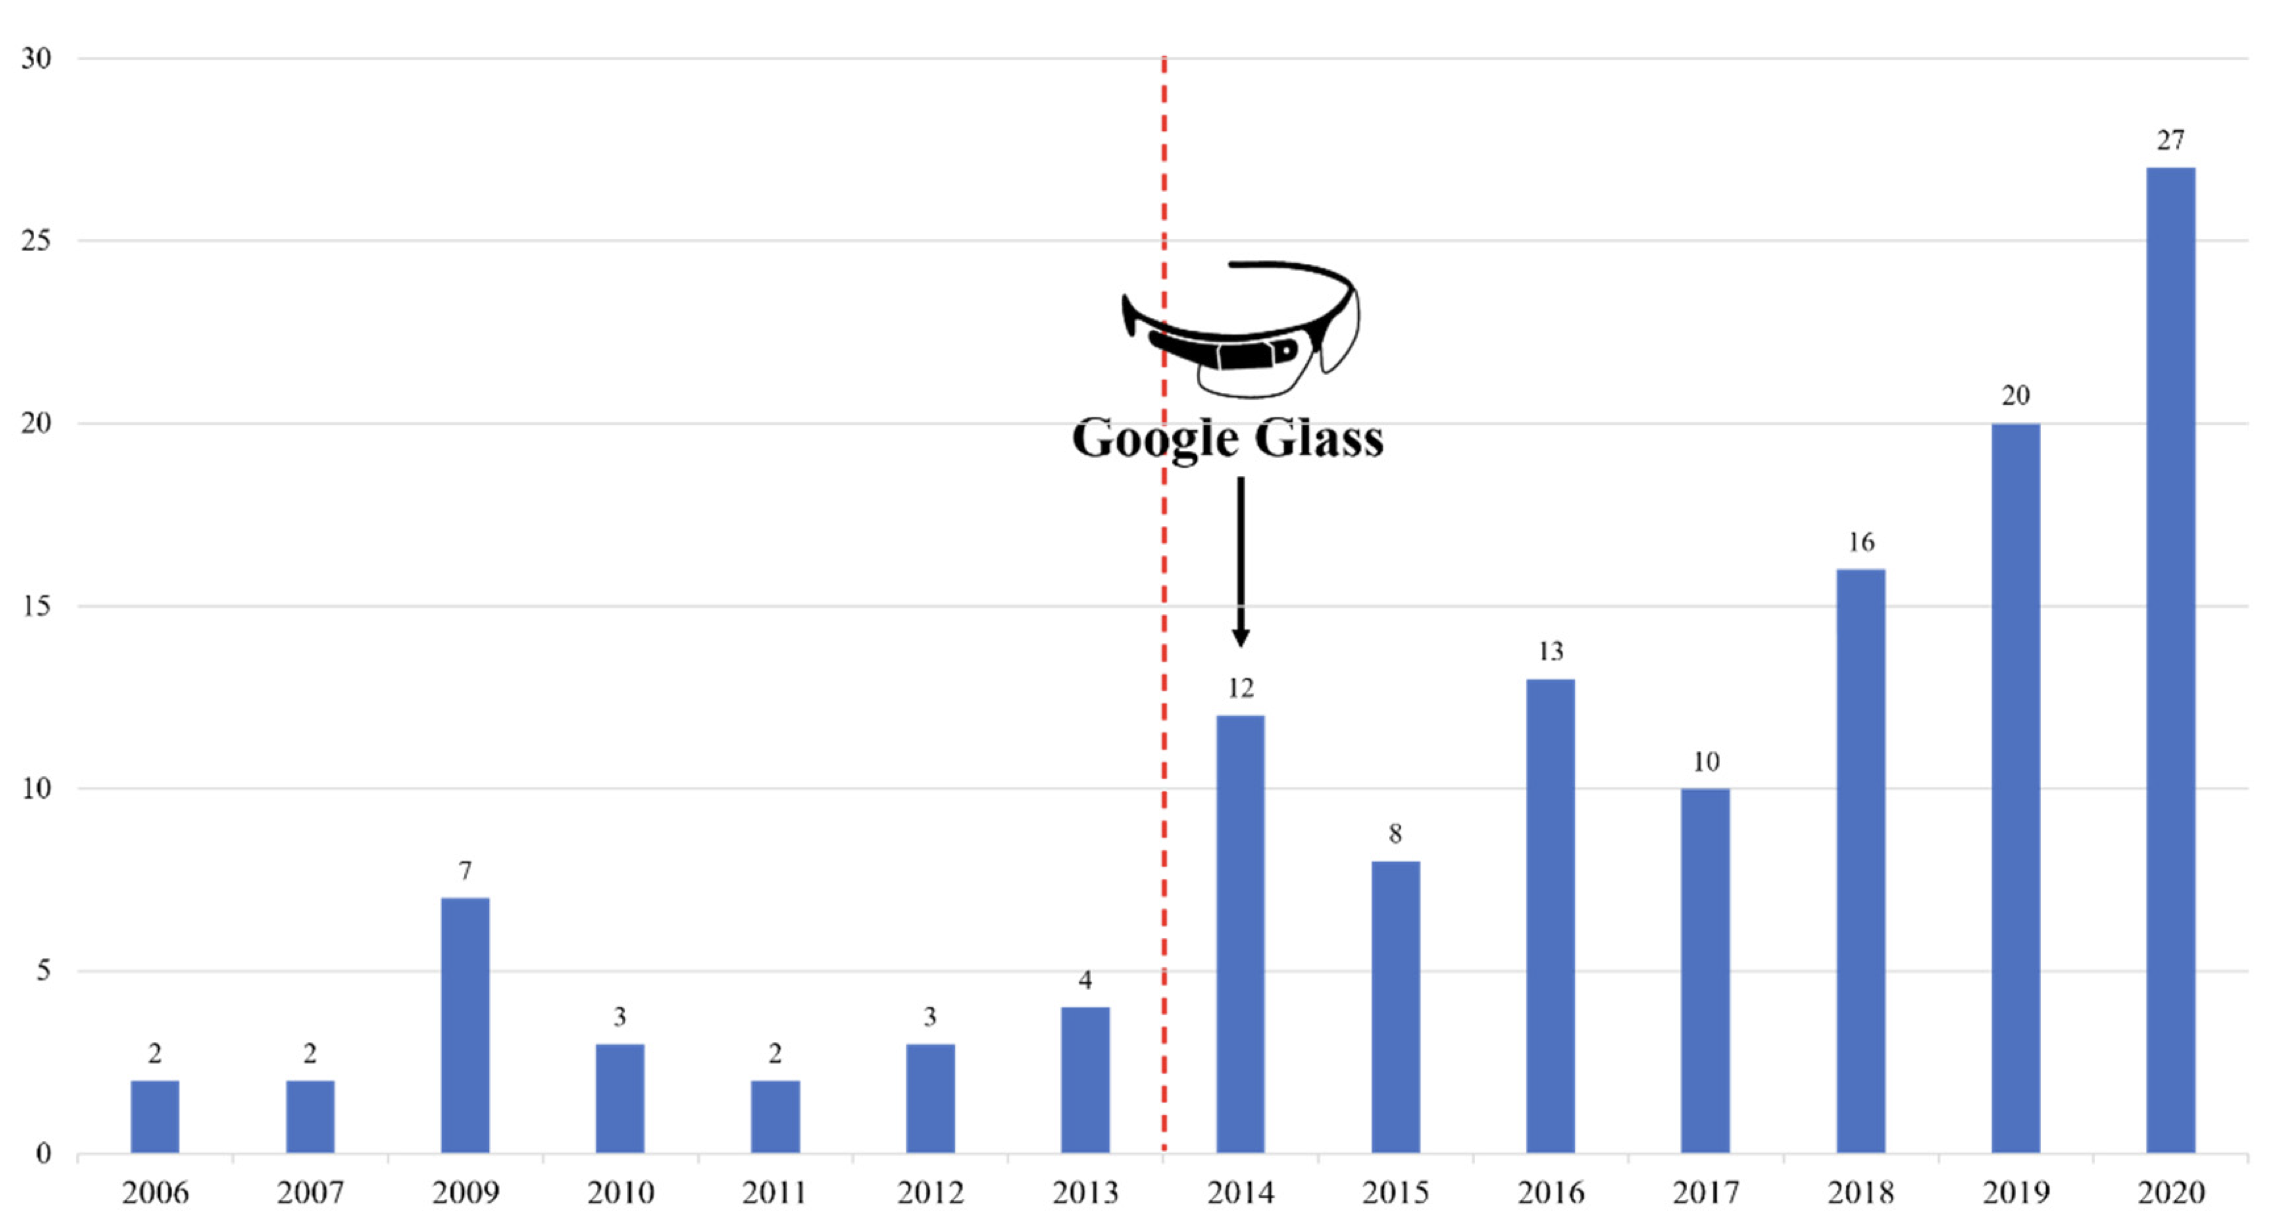
\includegraphics[scale=0.2]{img/entwicklung.png}}
    \caption{Anzahl an Paper über AR in der Bildung}
    \label{fig1}
\end{figure}

\section{Tools und Plattformen}\label{AA}
Damit AR in der Bildung funktionieren kann, müssen einige Kriterien erfüllt sein. Das Zusammenspiel
zwischen Software und Hardware ist essenziell, um eine immersive und interaktive Lernerfahrung
zu ermöglichen. Moderne Software ermöglicht es, Laborexperimente oder geschichtliche Ausflüge
zu veranstalten. Damit dies nahtlos in den Unterricht integriert werden kann, ist es wichtig, passende Hardware zu unterstützen.
Im Folgenden wird darauf eingegangen und an einigen realen Beispielen diskutiert.

\subsection{Software}
Damit die Software in den Bildungssektor passt, müssen Kriterien wie eine einfache Bedienung,
weite Verbreitung, geringe Kosten und passender, unterstützter Inhalt gewährleistet sein. Momentan
vorhandene Beispiele sind unter anderem:
\begin{itemize}
    \item \href{https://sites.google.com/dublinschools.net/vr-ar/google-geo-tools/google-expeditions}{Google Expeditions}
    \item \href{https://koerber-stiftung.de/projekte/eustory/teaching-and-learning-in-the-metaverse/}{Metaverse}
    \item \href{https://www.4danatomy.com/}{Anatomy 4D}
    \item \href{https://www.labster.com/}{Labster}
    \item \href{https://www.cospaces.io/}{CoSpaces Edu}
\end{itemize}
Jedes dieser Beispiele fokussiert sich auf einen speziellen Fachbereich
in der Bildung. Während Google Expeditions sich auf virtuelle sowie augmentierte
Erlebnisse und Ausflüge fokussiert, passt sich unter anderem Anatomy 4D speziell
auf die Lehre der Biologie im Bereich Anatomie von Mensch und Tier an. 
Labster ermöglicht es, Laborumgebungen zu augmentieren und so 
völlig neue Lernumgebungen zu schaffen. Mithilfe von CoSpaces Edu lässt sich unter 
anderem das Zusammenarbeiten trotz Distanz ermöglichen, indem andere Personen und 
Räume in den eigenen augmentiert werden können. \cite{w1}

\subsection{Hardware}
Damit die Hardware in den Bereich Bildung passt, muss auf einige Kriterien geachtet werden.
Unter anderem sollte, vor allem in der Benutzung im primären Bildungssektor, auf eine günstige Hardwareoption geachtet werden. Diese sollte einfach zu bedienen sein und nicht zu zerbrechlich sein.
In der Schule sind für diese Anwendung vor allem bereits vorhandene Hardware zu betrachten, zum Beispiel
LiDAR-fähige Tablets sowie Smartphones und Computer, die im Sinne der Schule bereits in das Curriculum
integriert sind. Diese benötigen teilweise keine weiteren Anschaffungskosten und auch keine weitere Schulung und Weiterbildung der Lehrkräfte und Schüler. 

Im Hinblick auf Bildung in der Hochschule und Weiterbildung in der Industrie sind vor allem kostenintensivere,
aber auch immersivere Hardwareoptionen möglich. Darunter gehören AR-Brillen und Headsets im Sinne von HUP (Head-up-Display),
Optical See Through und Visual See Through. Des Weiteren gibt es speziell auf Bildung angepasste Hardware wie der 
\href{https://mergeedu.com/cube?cr=4646}{Merge Cube}, welcher es ermöglicht, Schülern 3 dimensionale Objekte in die Hand zu
legen und damit zu interagieren. \href{https://zspace.com/}{ZSpace} hingegen ermöglicht es dem Anwender, mithilfe eines Stylus ähnlichen Stiftes, Objekte aus dem Monitor zu ziehen und diese zu manipulieren. \cite{b12}

Zu den wichtigsten Beispielen gehören unter anderem:
\begin{itemize}
    \item \href{https://www.microsoft.com/de-de/hololens}{Microsoft HoloLens} Abb. \ref{fig2}
    \item \href{https://www.meta.com/de/quest/quest-3/}{Meta Quest 3}
    \item \href{https://www.apple.com/de/apple-vision-pro/}{Apple Vision Pro}
\end{itemize}

Während das Microsoft HoloLens auf Optical See Through setzt, benutzen beide anderen Beispiel Video See Through, durch welche
zwar immersivere Erlebnisse gestaltbar sind, jedoch auch Nachteile durch Übelkeit möglich sind.

\begin{figure}[htbp]
    \centerline{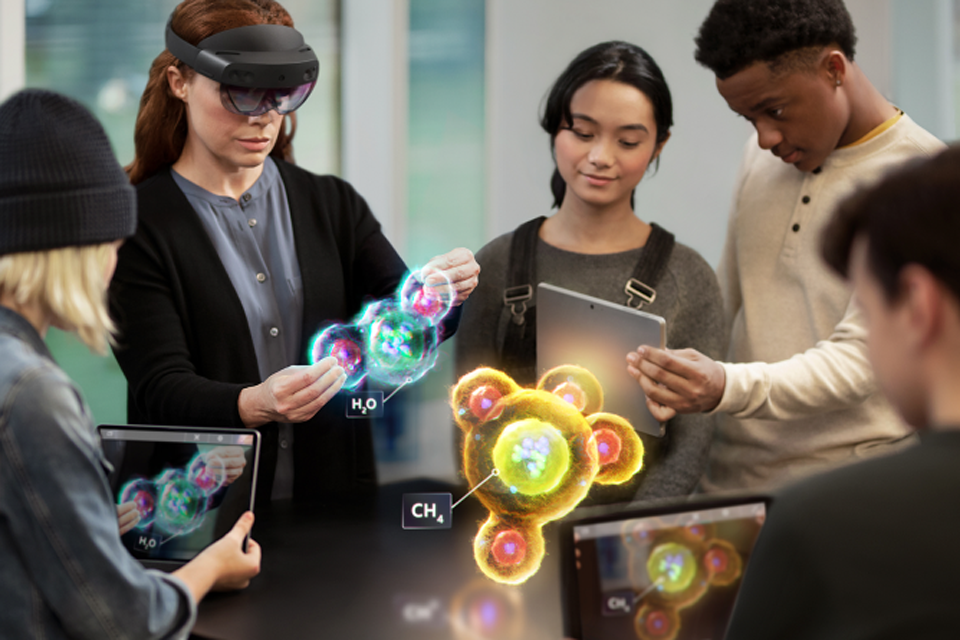
\includegraphics[scale=0.2]{img/holo.png}}
    \caption{HoloLens mit Hologrammen von Molekülen \cite{w3}}
    \label{fig2}
\end{figure}


\section{Virtuelle Räume}
Gerade seit der Covid-19-Pandemie ist auch das Thema der virtuellen Klassenräume interessant geworden.
Dabei ist zu unterscheiden zwischen dem virtuellen Klassenraum vor Ort und dem von anderen Orten aus.
Das Konzept besteht darin, dass entweder der Klassenraum an sich durch AR erweitert wird und somit der Unterricht
immersiv bereichert wird oder, dass der Klassenraum vollkommen in einen anderen Raum augmentiert wird und somit
ein authentischer Unterricht von anderen Orten möglich ist.

\subsection{vor Ort}
Die klassische und intuitive Art, AR in den Klassenraum einzubauen, ist die Art der Anwendung vor Ort.
Der Zweck eines virtuellen Klassenraums vor Ort besteht darin, dass gemeinsam in Präsenz die Nutzung von AR-Hardware in den bestehenden Unterricht eingebaut wird. 
Dies kann auf unterschiedliche Weise genutzt werden. Dazu gehört die Funktionsweise 
als unterstützende Aufgabe während des Unterrichts. Das momentan besprochene Thema kann durch Simulationen und Rendering von Modellen visualisiert werden. 
Des Weiteren können parallel kleinere Aufgaben in Form von spielerischen Ansätzen veranstaltet werden,
um die Motivation und Gedächtnisleistung während des Unterrichts anzuregen.
\subsubsection*{Probleme}
Zu den hier vorhandenen Problemen gehören vor allem die hohen Anschaffungskosten, die in vielen Schulsystemen nicht gerechtfertigt
werden können, sowie eine nötige Schulung des entsprechenden Personals. Zum Vergleich, eine Microsoft HoloLens 2 kostet für Bildungseinrichtungen
pro Exemplar rund \href{https://techcommunity.microsoft.com/t5/mixed-reality-blog/education-institutions-save-10-on-microsoft-hololens-2/ba-p/3282493}{3.500\$}.
Eine Meta Quest 3 kostet rund \href{https://www.meta.com/de/en/quest/quest-3/#}{500\$}, wobei es teilweise Abonnements gibt, die dies vergünstigen können.
\subsection{Remote}
Im Gegensatz zur Nutzung vor Ort bietet die Nutzung von AR von Zuhause oder anderen Orten (Remote) einige interessante Ansätze und Vorteile. 
Die Remote-Nutzung beinhaltet vor allem das Augmentieren einzelner Personen oder ganzer Räume in einen anderen, lokal gelegenen Raum \cite{b5}. Dies ermöglicht es, Fernunterricht, zum Beispiel aufgrund einer Quarantäne (individuell oder pandemisch bedingt)
oder aufgrund unzureichend vorhandener Infrastruktur (dazu gehören nicht genug vorhandene Schulen in abgelegenen Gebieten sowie 
beeinträchtigte Wege), durchzuführen. Dabei können Lehrer, optional Mitschüler und jegliche Unterrichtsmaterialien, in den eigenen Raum 
augmentiert werden, um ein lebendiges und authentisches Lernerlebnis auch außerhalb des Klassenraums zu ermöglichen.
\subsubsection*{Probleme}
Neben den auch hier sehr hohen Investitions- und Schulungskosten kommt das Problem dazu, dass diese Technologie noch nicht in einer 
anwendbaren Phase entwickelt wurde. Dazu gehört das Echtzeit-Scannen von Personen und ganzen Räumen sowie die Projektion in nicht vordefinierte Räume.

\section{Anwendungen}
Der Bereich AR in der Bildung lässt sich in 7 Bereiche einteilen (siehe Abb. \ref{fig3}).

\begin{figure}[htbp]
    \centerline{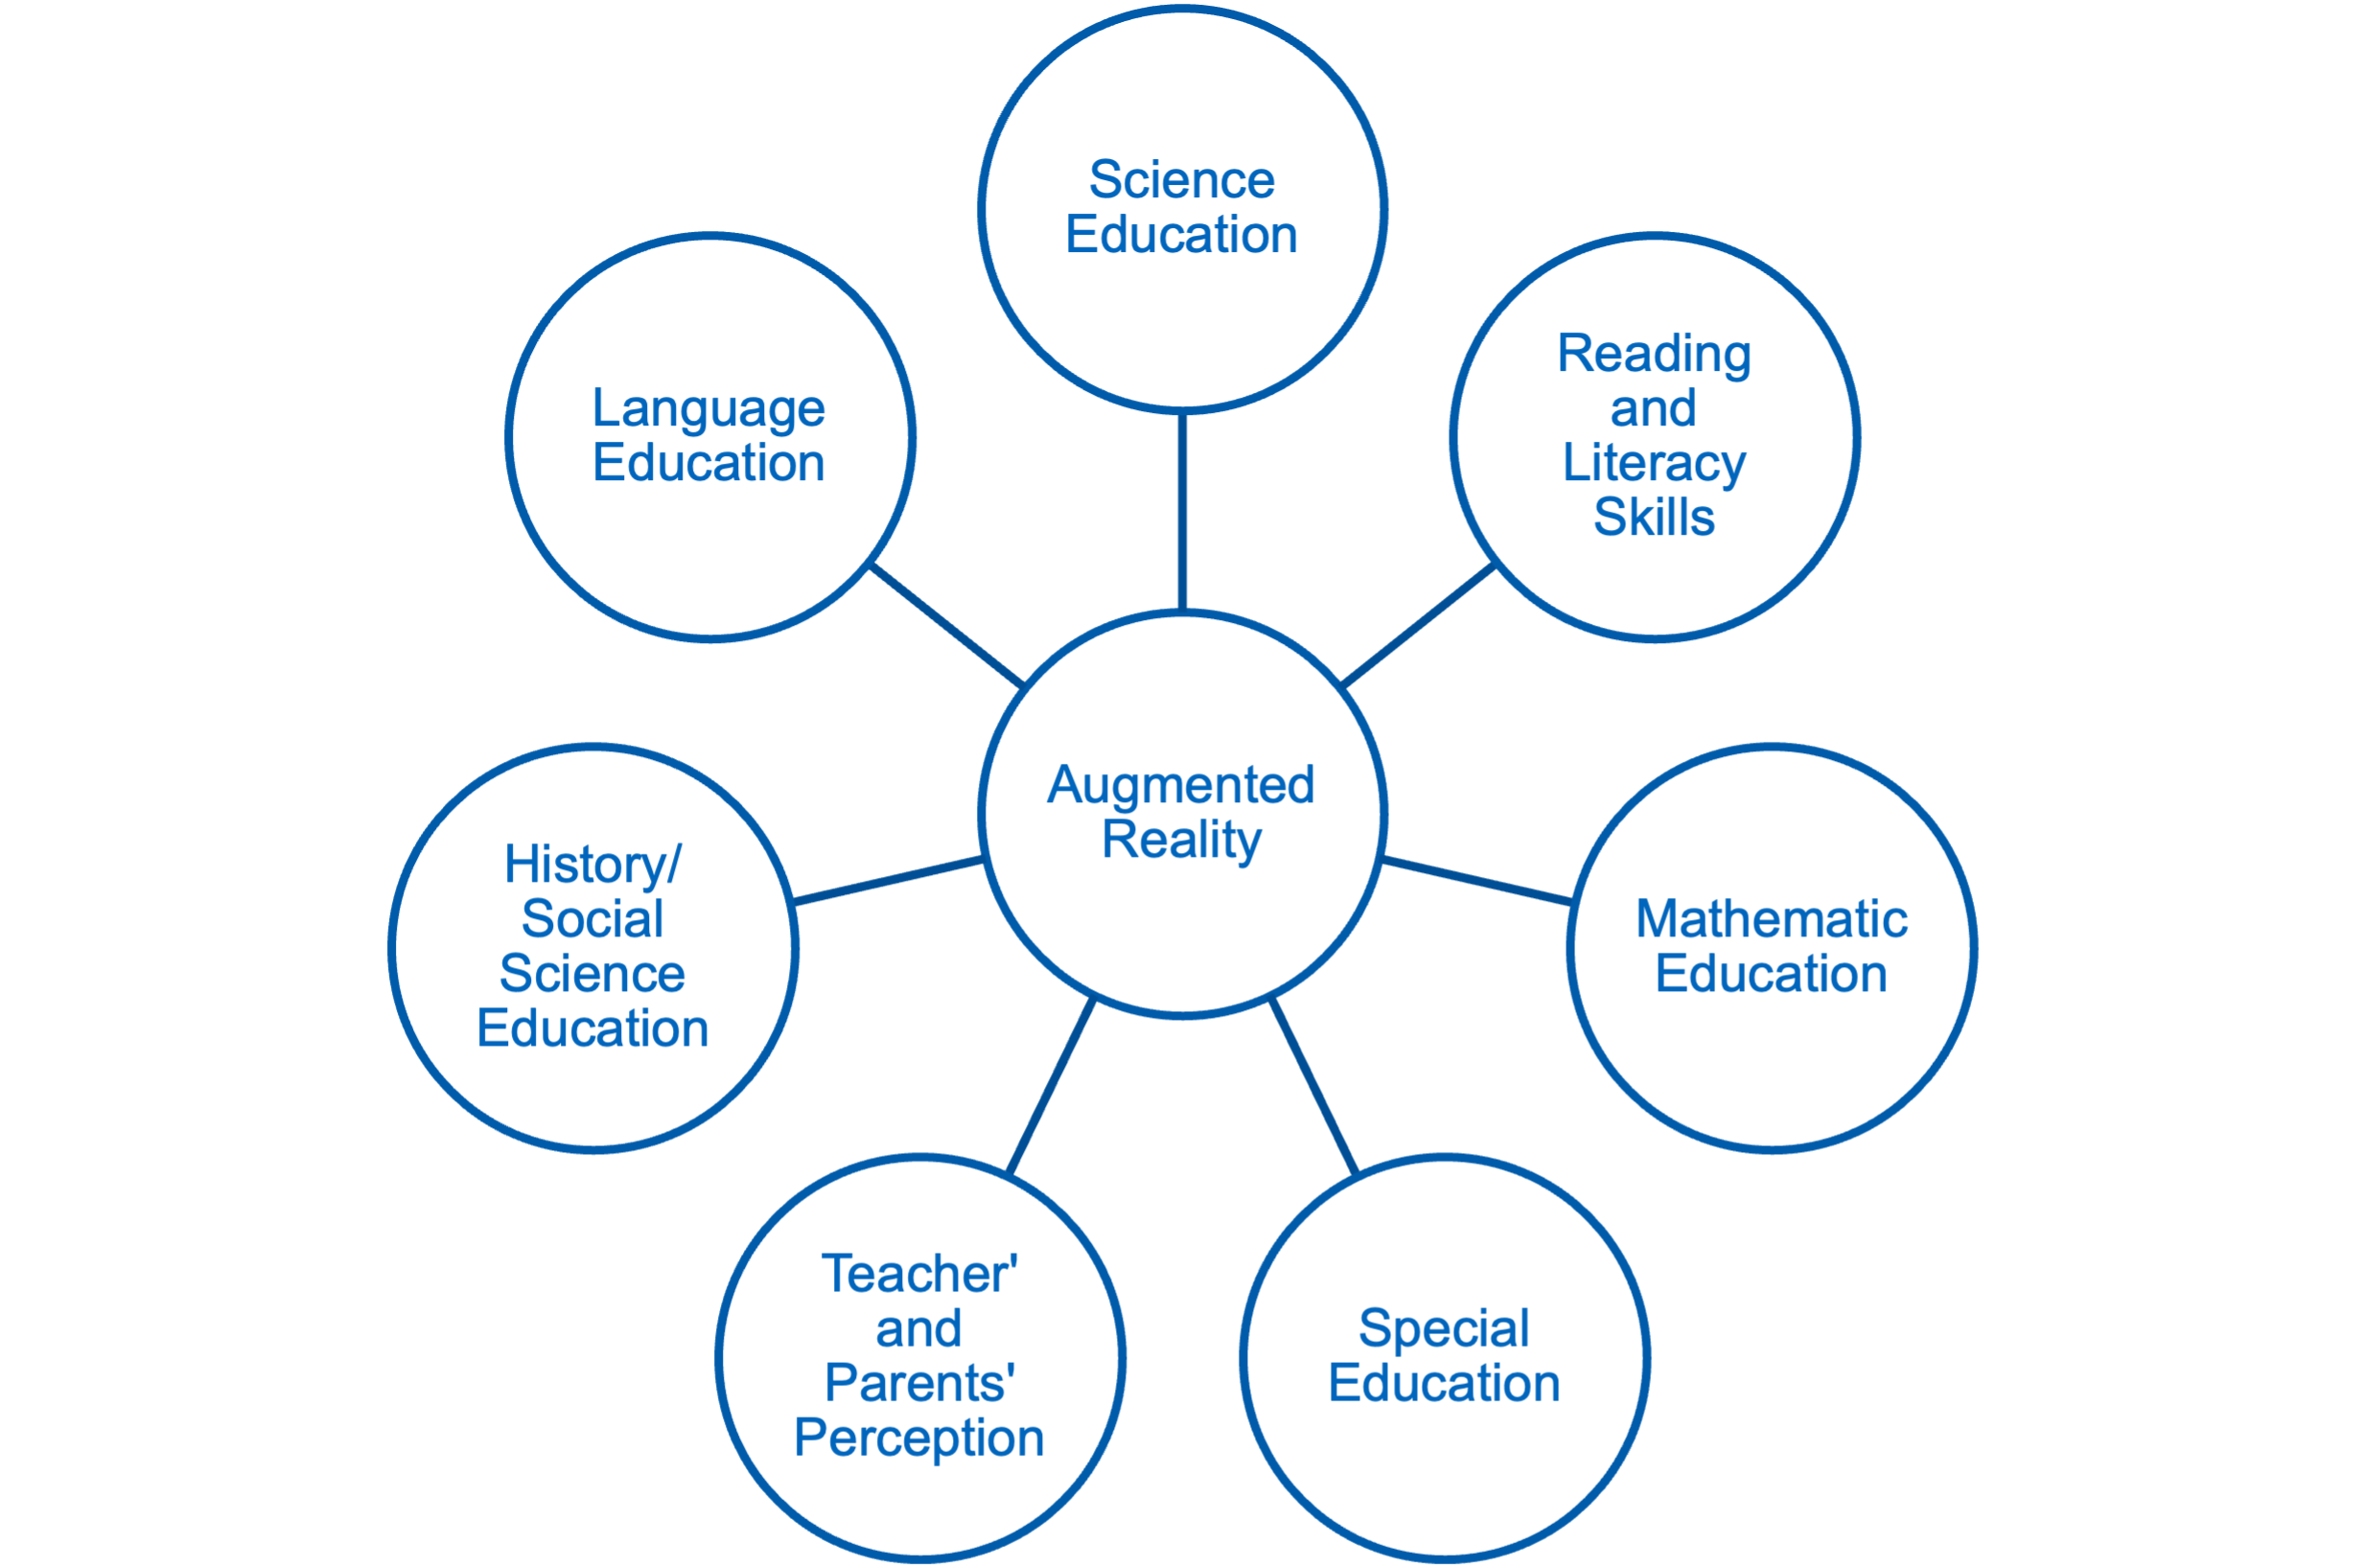
\includegraphics[scale=0.3]{img/sections.png}}
    \caption{Sektionen der Bildung \cite{b4}}
    \label{fig3}
\end{figure}

Während 5 dieser Sektionen mit den traditionellen Bildungsbereichen der Schulsysteme einhergehen, sind 
auch Themen wie Special Education (Bildung für Menschen mit Lernbehinderungen), sowie die Auswirkungen
und möglichen Ergebnisse der Anwendung, sowie die Wahrnehmung der Lehrkräfte und Eltern, relevant.

\subsection{Primär und Sekundär}
Im Folgenden wird die mögliche Anwendung von AR in den primären und sekundären Bildungsstufen behandelt.
Des Weiteren ist zu bemerken, dass mit ''K-12 Education'' (Begriff aus dem angloamerikanischen Raum) der Abschnitt von der Grundschule bis inklusive Sekundarstufe 1 beziehungsweise 2 gemeint ist. Die Integration von modernen AR-Technologien ermöglicht vielseitige Möglichkeiten, den Unterricht und das Lernen zu verändern und zu bereichern.

Die Anwendung von AR in der Grundbildung ist vor allem in Richtung ''Gamification'', 
also den spielerischen Ansätzen in Lernkontexten, um möglicherweise die Motivation und das Engagement von Schülerinnen
und Schülern zu steigern, zu betrachten. Augmented Reality kann es ermöglichen, sehr abstrakte und komplexe Lerninhalte durch interaktivere Erlebnisse für junge Schüler zugänglicher zu machen. Beispielsweise können vor allem einige mathematische Konzepte,
die oft schwer verständlich sind, durch Spiele und Simulationen visualisiert und dargestellt werden. Dadurch kann
neben den zu erwartenden Lernerfolgen auch das kreative Denken gefördert werden. \cite{b4}

Vor allem in den Naturwissenschaften kann AR eine innovative Möglichkeit sein, unterschiedliche Konzepte darzustellen.
Anwendungen können molekulare Strukturen, physikalische Phänomene oder biologische Prozesse in interaktiven Umgebungen darstellen, die weitaus effektiver sind als herkömmliche Lernmethoden. 
Darunter können vor allem Themen wie der Aufbau von Atomen oder die Funktionsweise und Aufbau des Nervensystems fallen (siehe Abb. \ref{fig2}). Dadurch können Lernende diese Konzepte nicht nur sehen,
sondern auch damit interagieren und diese erforschen. \cite{b6}

Des Weiteren können Anwendungen in der Augmented Reality für Projektarbeiten genutzt werden, in denen in einer kooperativen und interaktiven Lernumgebung Schülerinnen und Schüler gemeinsam digitale Modelle erstellen, erkunden und bearbeiten können.
Diese können dann den Mitschülern interaktiv präsentiert werden. Dies fördert nicht nur das Verständnis der gelehrten Inhalte,
sondern auch wichtige soziale Fähigkeiten, Kommunikation und Problemlösungsfähigkeiten.

\subsubsection*{Fallstudie}
Eine Fallstudie, welche eine mögliche Anwendung von AR im primären Bildungssektor untersucht hat, ist die Anwendung ''Cooking Math''.
Diese wurde an einer griechischen Grundschule testweise in das griechische Curriculum für Mathematik eingebaut und von einer Gruppe von Pädagogikstudenten und Ingenieursstudenten durchgeführt.
Die Anwendung erlaubt es den Schülerinnen und Schülern mithilfe eines Tablets verschiedene mathematische Konzepte und Aufgaben zu verstehen. Ziel ist es, mithilfe von ''Kochaufgaben'' (Abb. \ref{fig4}) einfache Aufgaben in den Themen Geometrie, den rationalen Zahlen und Gleichungen zu untersuchen und zu lösen.

\begin{figure}[htbp]
    \centerline{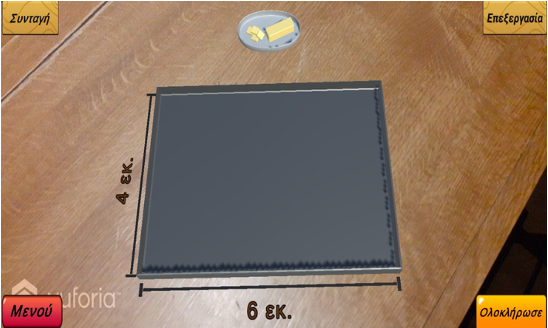
\includegraphics[scale=0.7]{img/geometrie.png}}
    \caption{Aufgabe im Bereich Geometrie \cite{b8}}
    \label{fig4}
\end{figure}

Die Ergebnisse der System Usability Scale (SUS) Fragebögen und Interviews waren überwiegend positiv. Die Schüler bewerteten das Erlebnis positiv, es wurden jedoch einige Verbesserungen vorgeschlagen. \cite{b8}

\subsection{Hochschule}
Die Anwendung von AR im Hochschulsektor bietet viele weitreichende Möglichkeiten. Die Technologien können auch in diesem Sektor die traditionellen
Lernmethoden erweitern und interaktivere Auseinandersetzungen mit komplexen Konzepten ermöglichen.

Ein bedeutsames Einsatzgebiet von AR ist das experimentelle Lernen, insbesondere in den Natur- und Ingenieurwissenschaften.
Durch AR können traditionelle Laborexperimente und Umgebungen erweitert und in die reale Umgebung integriert werden. Dadurch sind Experimente möglich,
welche nicht an die physischen Einschränkungen eines traditionellen Labors gebunden sind. Vor allem vorteilhaft sind diese in Situationen, bei denen
theoretische Kosten oder andere Komplikationen ein Hindernis stellen würden.\cite{b9} Somit können beispielsweise chemische Reaktionen, die normalerweise
aufgrund von Sicherheitsbedenken nicht möglich wären, in einer AR-Umgebung simuliert werden. Ebenso ist es möglich, interaktive Modelle für Ingenieurstudenten zu entwickeln, welche bei der Lehre helfen sollen. Abb. \ref{fig5}

\begin{figure}[htbp]
    \centerline{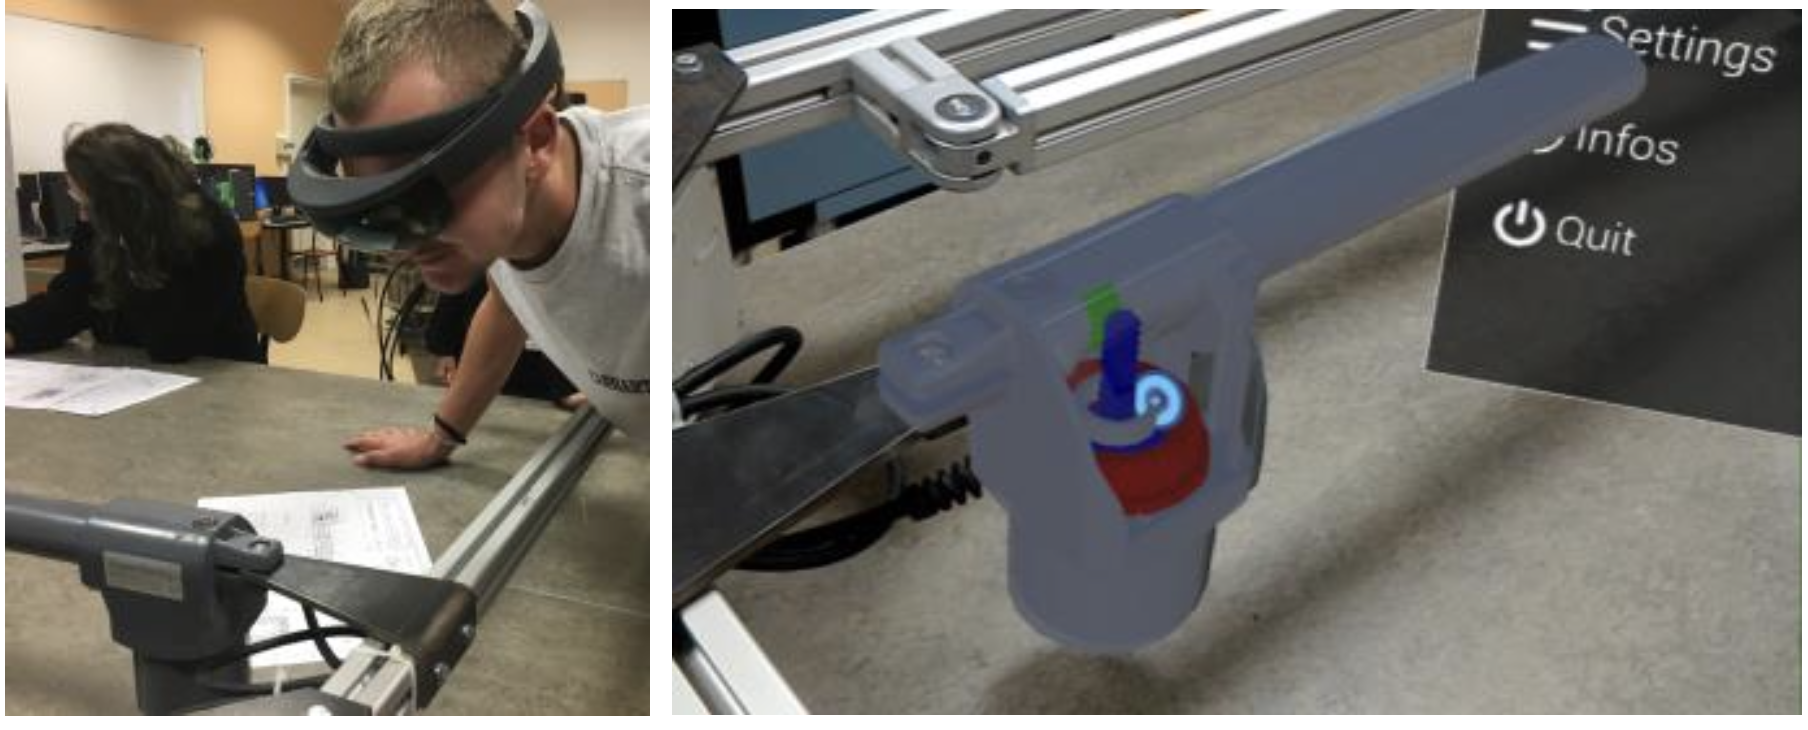
\includegraphics[scale=0.25]{img/ingen.png}}
    \caption{AR CAD mit HoloLens \cite{b9}}
    \label{fig5}
\end{figure}

Neben dem experimentellen Lernen im Hochschulsektor, gibt es auch neue Wege für allgemeinere Studiengänge, komplexe Konzepte visuell besser darstellen zu können.
Vor allem in der Medizin ist es möglich, anatomische Strukturen und physiologische Prozesse durch AR interaktiver und verständnisvoller darstellen zu können.
Hierbei können virtuelle Modelle des menschlichen Körpers erkundet werden (siehe Demo \ref{demo}) oder Operationen simuliert werden, bevor diese in tatsächlichen klinischen Umgebungen gemacht werden. 
\cite{b10} Auch möglich sind Interaktionen in den Geowissenschaften, bei denen tektonische Verschiebungen, geologische Formationen oder andere Klimamodelle erkundbar werden.

\subsubsection{Fallstudie}
An der University of Edinburgh's Medical School wurde das Projekt ''EdAR'' verwirklicht, welches das Unterrichten von X-Ray Methoden an komplexen Körperteilen,
wie zum Beispiel dem Becken, vereinfachen soll. \cite{b11} Dabei wird ein 3D-Modell eines Beckenknochens aufgestellt. Mithilfe eines Markers kann das 3D-Modell mit einem Smartphone oder Tablet gescannt werden, woraufhin die axialen, coronalen und sagittalen Ebenen angezeigt werden, welche auch modifiziert werden können. Des Weiteren
kann nach dem Einstellen ein mögliches X-Ray Ergebnis angezeigt werden. Abb. \ref{fig6}

\begin{figure}[htbp]
    \centerline{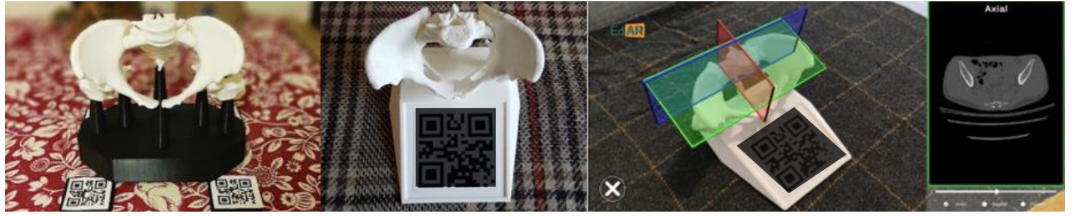
\includegraphics[scale=0.45]{img/bone.png}}
    \caption{Modell eines Beckenknochens \cite{b11}}
    \label{fig6}
\end{figure}

Aufgetretene Limitierungen sind vor allem das Problem der zu kleinen Bildschirme der Smartphones und Tablets, welche die Sicht einschränken können. Trotzdem ist diese 
Fallstudie ein gutes Exemplar, welches zeigt, wie Augmented Reality in der Hochschulbildung eingesetzt werden kann.

\subsubsection{Fallstudie}
Aufgrund der durch COVID-19 eingeschränkten Studienmöglichkeiten am Imperial College in London konnten Studierende lange Zeit an keinen Untersuchungen der Ärzte teilnehmen. \cite{w4}
Mittels der Augmented-Reality-Brille HoloLens wurde unter Einverständnis der Patienten die Untersuchung aufgenommen, damit diese in Echtzeit an die Studierenden übertragen werden kann. Dadurch war es möglich, trotz der Einschränkungen, einen virtuellen Überblick der Behandlung zu bekommen. Gleichzeitig konnten Krankenakten sowie Röntgenbilder
auf der Augmented Reality Brille übertragen werden, welche zur möglichen Diagnose direkt hinzugezogen werden konnten. Abb. \ref{fig7}

\begin{figure}[htbp]
    \centerline{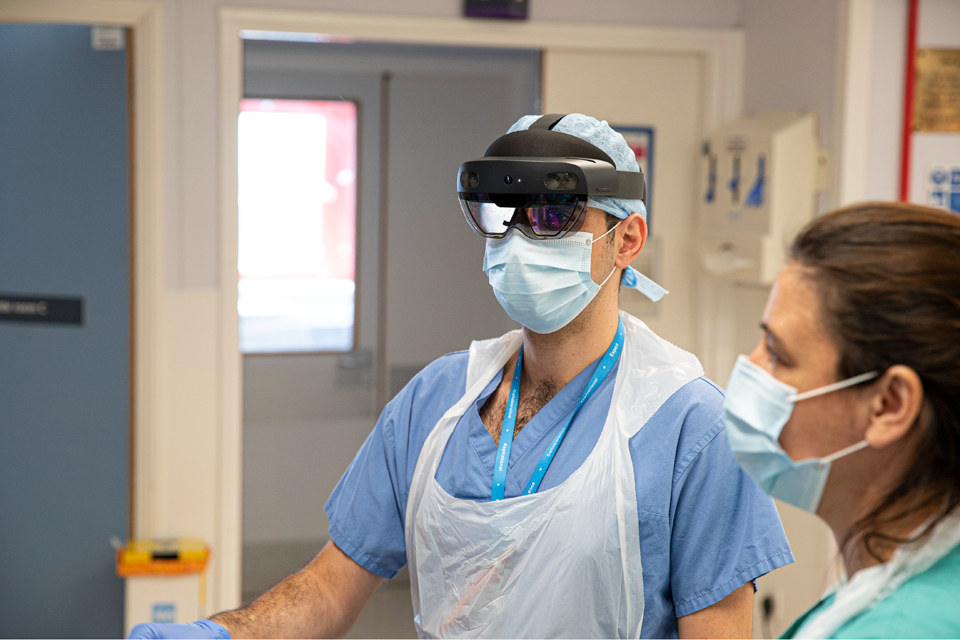
\includegraphics[scale=0.2]{img/med.png}}
    \caption{HoloLens in der Universitätsklinik des Imperial College \cite{w4}}
    \label{fig7}
\end{figure}

\section{Weiterbildung}
Auch in der Industrie hat die Bildung eine wichtige Stellung, um die Mitarbeitenden auf verschiedenste Weisen weiterbilden zu können.

Durch AR ist es möglich, Schulungsinhalte direkt am Arbeitsplatz zu vermitteln. Teilnehmende können Anweisungen mithilfe von AR-Headsets oder Smartphones in Echtzeit erhalten,
um so in Bereichen wie der Wartung und Instandhaltung von größeren Geräten unterstützt und geschult zu werden.

Da die Weiterbildung sehr stark mit dem eigentlichen Nutzen von AR in der Herstellung und Bearbeitung zusammenhängt, wird nicht weiter darauf eingegangen.

\section{Potenzial}
Wie durch die weitreichenden Anwendungsmöglichkeiten bereits gesehen, birgt die Anwendung von AR in den verschiedensten Bildungsbereichen eine Menge Potenzial.
Die Möglichkeit, traditionelle Lernmethoden auf moderne Weise, mit pädagogischem Hintergrund, zu erweitern, kann das Lernverhalten und die Resultate in Zukunft erheblich verändern. Potenzial ist zum einen in dem personalisierten Lernen zu finden, welches basierend auf den Fortschritten, den Lernstil sowie das Lerntempo individuell anpassen kann. Dazu gehört auch das Anpassen an barrierefreie Situationen, damit Schülerinnen und Schüler mit Beeinträchtigungen ähnliche Lernerfahrungen machen können.
Auch die möglichen virtuellen und kulturellen Immersionen können einen weitaus größeren Teil des Curriculums spielen, um auch Erfahrungen zu machen, die nicht in unmittelbarer Nähe liegen.

Interdisziplinäre Lernumgebungen ermöglichen es, verschiedenste Fachbereiche zu verknüpfen. Durch neue Umsetzungsmöglichkeiten können Schülerinnen und Studierende auch Projekte in Kombination mit anderen Themenbereichen durchführen. 
Vor allem jedoch das Remote-Lehren hat viel Potenzial, da dieses heutzutage erst sehr begrenzt behandelt und unterstützt wird. Die Möglichkeit, immersive Lernerfahrungen auch außerhalb des Klassenraums zu erleben, bietet vielen Leuten mehr Flexibilität, Freiheit und kann einigen Menschen erst die Bildung überhaupt ermöglichen. 

Auch mögliche Prüfungen können durch Augmented Reality verändert und verbessert werden.

\section{Fazit}
Trotz dieser Vorteile gibt es immer noch eine Menge Probleme und Hürden. Neben den bereits genannten sehr hohen Investitionskosten, die nicht nur den noch nicht komplett ausgereiften
und noch immer eher seltenen Hardwareoptionen, sondern auch der breiten Bereitstellung und Schulung von Personal zu verschulden ist, ist das Thema der AR Bildung noch ein nicht sehr
breit erforschter Bereich. Viele mögliche Potenziale wurden noch nicht ausgetestet oder werden erst gar nicht in Betracht gezogen. Dazu zählt vor allem die fehlende Digitalisierung 
an vielen Schulen und die nicht vorhandene Bereitschaft, in diese zu investieren. Außerdem ist der tatsächliche Lerneffekt von AR noch nicht wirklich untersucht worden. Die meisten Fallstudien beziehen sich auf kurzweilige Projekte von wenigen Tagen bis Wochen, in denen kein nennenswerter Erfolg gewährleistet werden kann. Um tatsächliche, stichfeste Ergebnisse in dem Bereich zu bekommen, würde sich ein Pilotprojekt lohnen, in dem Schülerinnen und Schüler gezielt mindestens ein ganzes Schuljahr teilweise oder komplett in Unterstützung von AR den Unterricht durchführen.
Die Ergebnisse von gegebenenfalls vorhandenen Tests können dann mit Schülern anderer Klassen ohne das jeweilige Pilotprojekt verglichen werden.

Augmented Reality in der Bildung ist zusammengefasst ein breites Thema, welches viel Potenzial birgt, welches jedoch bis heute noch nicht vollkommen ausgenutzt und untersucht wird.
Fallstudien zeigen eine mögliche breite Akzeptanz und viele verschiedene Anwendungsmöglichkeiten. Um diese noch weiter ausschöpfen zu können, muss es in Zukunft gewagtere Projekte, 
bessere Investitionsmöglichkeiten und mehr Forschung geben.

\section{Demo}
\label{demo}
Im Zusammenhang mit diesem Paper wurde eine Live-Demo mithilfe von \href{https://ar-js-org.github.io/AR.js-Docs/}{AR.js} entwickelt, welche die Anatomie eines menschlichen 
Körpers als 3D Modell inklusive passender Beschriftung zeigt. Das Projekt kann auf diesem \href{https://lydr.io/ar}{Link} mit folgendem \href{https://lydr.io/ar/hiro.png}{Marker} selber getestet werden.


\begin{thebibliography}{00}
    \bibitem{b1}  M. Dunleavy, C. Dede, and R. Mitchell, ''Affordances and Limitations of Immersive Participatory Augmented Reality Simulations for Teaching and Learning''. Journal of Science Education and Technology, 2009.
    \bibitem{b2} M. E. C. Santos, A. Chen, T. Taketomi, G. Yamamoto, J. Miyazaki, and H. Kato, ''Augmented Reality Learning Experiences: Survey of Prototype
    Design and Evaluation''. IEEE Transactions on Learning Technologies, 2014.
    \bibitem{b3} J. Bacca, S. Baldiris, R. Fabregat, S. Graf, and Kinshuk, ''Augmented Reality Trends in Education: A Systematic Review of Research and Applications''. Educational Technology and Society, 2014.
    \bibitem{b4} H. Cetin, “A Systematic Review of Studies on Augmented Reality Based Applications in Primary Education”, IJELS, 2022.
    \bibitem{b5} J. Zhang, G. Li, Q. Huang, Q. Feng and H. Luo, „Augmented Reality in K–12 Education A Systematic Review and Meta-Analysis of the Literature from 2000 to 2020”, MDPI, 2022.
    \bibitem{b6} M. Akçayır, and G. Akçayır, ''Advantages and challenges associated with augmented reality for education: A systematic review of the literature''. Educational Research Review, 2017.
    \bibitem{b7} P. Chen, X. Liu, W. Cheng and R. Huang, ''A review of using augmented reality in education from 2011 to 2016''. Innovations in Smart Learning, 2017.
    \bibitem{b8} C. Volioti, O. Christos, T. Sapounidis, G. Trachanas and E. Keramopoulos, ''Augmented Reality in Primary Education: An Active Learning Approach in Mathematics''. Computers, 2023.
    \bibitem{b9} D. Scaravetti, D. Doroszewski, ''Augmented Reality experiment in higher education, for complex system appropriation in mechanical design''. 29th CIRP Design Conference, 2019
    \bibitem{b10} O. George, J. Foster, Z. Xia and C. Jacobs, ''Augmented Reality in Medical Education: A Mixed Methods Feasibility Study''. Cureus, 2023.
    \bibitem{b11} D. Korre, and A. Sherlock, ''Augmented Reality in Higher Education: A Case Study in Medical Education''. Immersive Learning Research - Practitioner, 2023.
    \bibitem{b12} M. Vásquez-Carbonell, ''A Systematic Literature Review of Augmented Reality in Engineering Education: Hardware, Software, Student Motivation and Development Recommendations''. Digital Education Review, 2022.
\bibitem[w1]{w1} \href{https://www.cospaces.io/tech-check-ar-with-smartphones}{https://www.cospaces.io/tech-check-ar-with-smartphones} letzter Zugriff 07.07.2024 16:32
\bibitem[w2]{w2} \href{https://www.marketresearchfuture.com/reports/ar-vr-in-education-market-10834}{https://www.marketresearchfuture.com/reports/ar-vr-in-education-market-10834} letzter Zugriff 03.07.2024 20:38
\bibitem[w3]{w3} \href{https://news.microsoft.com/de-de/hololens-hologramme-in-lehre-und-forschung/}{https://news.microsoft.com/de-de/hololens-hologramme-in-lehre-und-forschung/} letzter Zugriff 27.08.2024 18:54
\bibitem[w4]{w4} \href{https://www.imperial.ac.uk/news/197617/mixed-reality-headsets-hospitals-help-protect-doctors/}{https://www.imperial.ac.uk/news/197617/mixed-reality-headsets-hospitals-help-protect-doctors/} letzter Zugriff 27.08.2024 19:03
\end{thebibliography}
\vspace{12pt}

\end{document}
